
\section{Introdução}

\par A programação web vem ganhando cada vez mais espaço na mundo globalizado, nos dias atuais torna-se praticamente inviável a instituições dos mais variados tipos, que não possuem um web sitio e neste aspecto que se capacita profissionais para este leque.
\par Segundo \citeonline{alvaron:2024}, empreas que não possuem site perdem clientes para concorrentes, pois sem um site os sites de pesquisas não irão encontrar a empresa para aquisição de algum ou alguns produtos ou serviços.




\section{Métodos}
\par Para esta aula prática foi proposto um roteiro, está disposto em: \href {https://github.com/ENGENHARIA-DE-SOFTWARE-UNOPAR/web-project/blob/main/Roteiro%20aula%20pr%C3%A1tica.pdf} {roteiro da aula prática}. De igual modo cria-se um repositório no GitHub para o versionamento da referiada aula prática, e que pode ser acessado atráves deste \href {https://github.com/ENGENHARIA-DE-SOFTWARE-UNOPAR/web-project} {link}.
\par Neste vies foi eleito o modelo de relatórios em \textbf{LaTeX}, pois o mesmo acaba automatizando alguns aspectos. Nos aspectos da realização de atividade foi sugerido a utilização da IDE \textbf{Eclipse}, a instalação do \textbf{}{Postman} e como opcional o \textbf{Git}. Porém opto pela utilização da IDE \textbf{VS Code}, pois a mesma já vem integrado \textit{plugin} do \textbf{Postmam}, conforme demonsstra a figura \ref{fig:pos}.

\begin{figure}[H]
\center
  \caption{Plugin do Postman na IDE vscode.}
  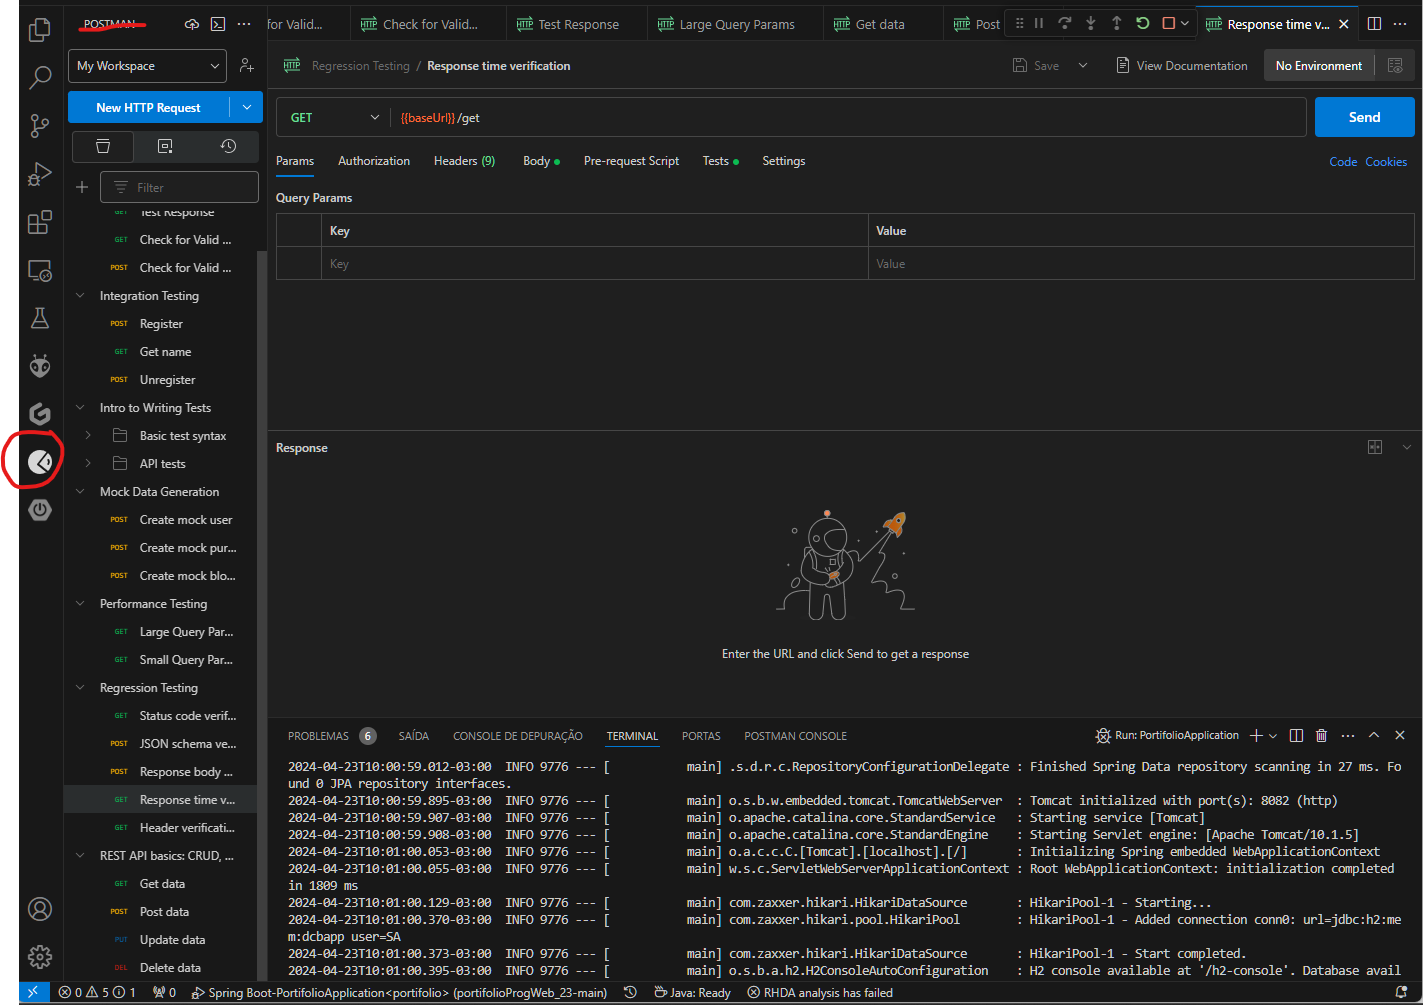
\includegraphics[width=\textwidth]{figure/postman_vscode.png}
  \label{fig:pos}
  \flushleft %esquerda
    {\fontsize{10pt}{\baselineskip}\selectfont
    Fonte: O autor (\the\year) }
\end{figure}

\par Sugere a criação de um modelo pré configurado através da ferramenta \textit{\textbf{Spring initialir}}, e a pré configuração foi definida conforme demontrada na figura \ref{fig:spring}. a versão do \textit{Spring} definida no roteiro é a \textbf{3.0.0}, no entanto não esta mais disponível e optei pela versão \textbf{3.2.5}.


\begin{figure}[H]
\center
  \caption{Configuração Spring initialir}
  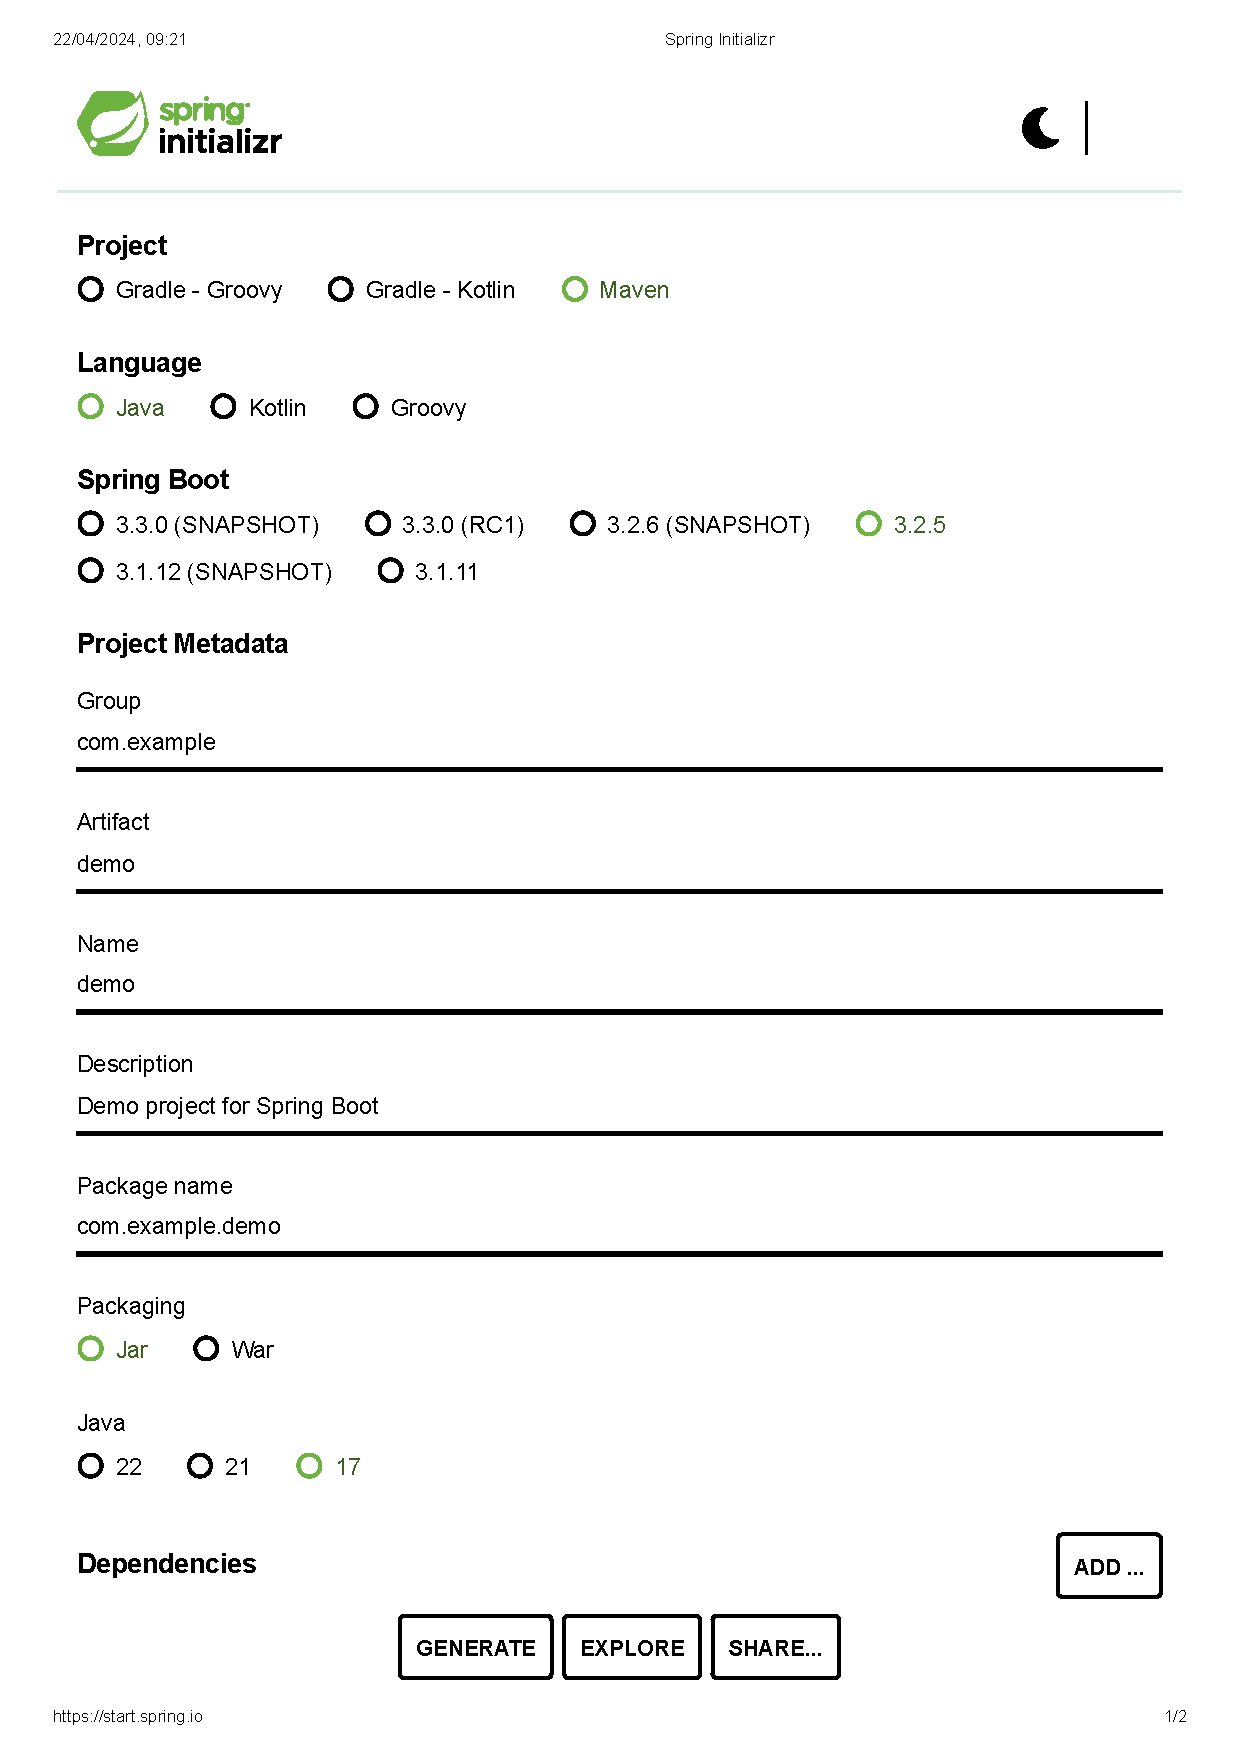
\includegraphics[width=\textwidth]{figure/Spring Initializr.pdf}
  \label{fig:spring}
  \flushleft %esquerda
    {\fontsize{10pt}{\baselineskip}\selectfont
    Fonte: O autor (\the\year) }
\end{figure}


\par É realizado uma sequência de passos disponibilizada no roteiro, e em relação ao passo \textbf{7}, que indica a criação de um arquivo chamado de \textit{application.properties}, já estava criado. com o conteúdo \textbf{(spring.application.name=demo)}, e então apenas adicionei abaixo o conteúdo indicado no roteiro.



\section{Resultados}
\par Após as implementações e alguns problemas, foi prosseguido para os testes, na figura \ref{fig:com} de monsta o resultado da compilação do código em java.

\begin{figure}[H]
\center
  \caption{Resultado da compilação do código em Java.}
  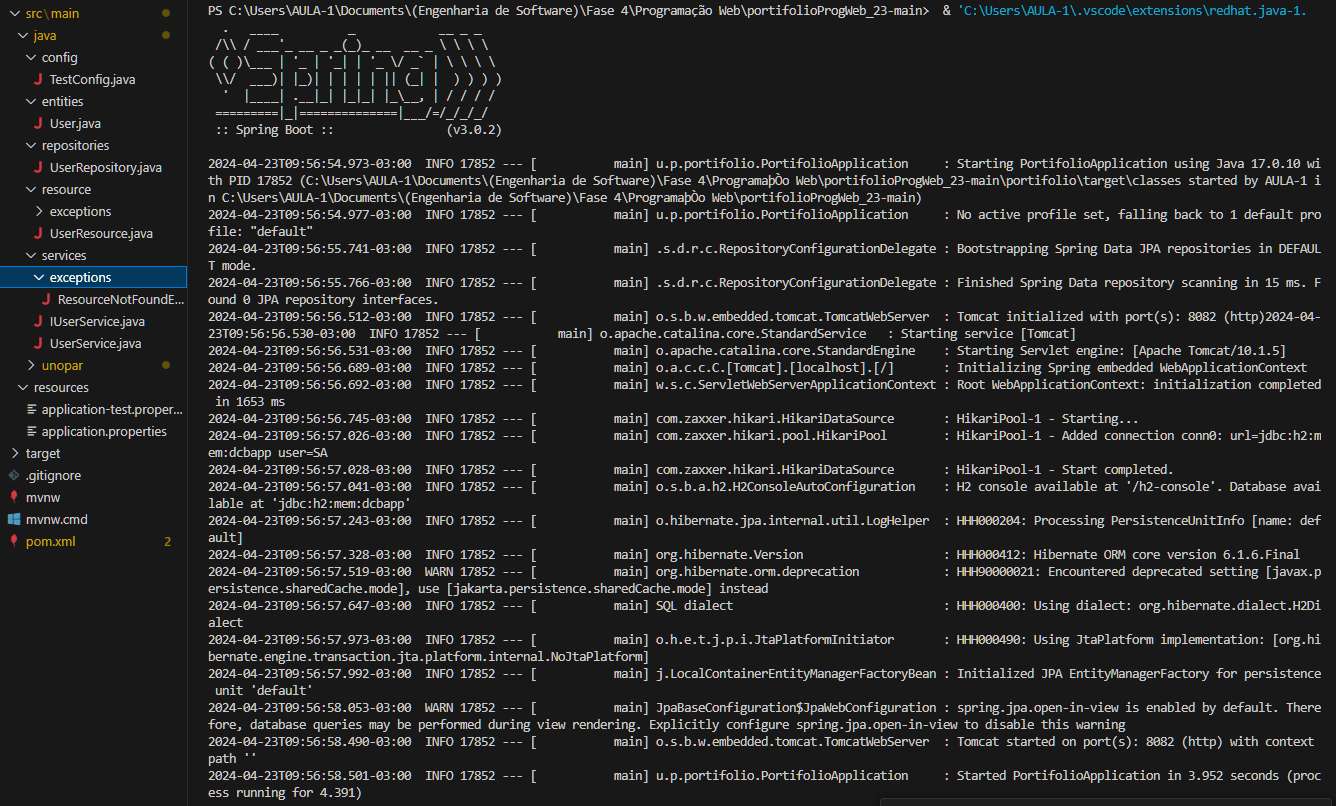
\includegraphics[width=\textwidth]{figure/resultado da compilação.png}
  \label{fig:com}
  \flushleft %esquerda
    {\fontsize{10pt}{\baselineskip}\selectfont
    Fonte: O autor (\the\year) }
\end{figure}

\par Nesta compilação pode-se averiguar o nome para acesso e a porta de escuta, o nome para acesso é \textbf{h2-console}, conforme defenido no \textbf{pom.xml} e a porta de escuta é a \textbf{8082}.

\par Realizo dois teste no \textbf{postman}, um com o \textbf{GET} e outro com o \textbf{POST}, demonstrado nas figuras \ref{fig:get} e figura \ref{fig:post}, sequencialmente.

\begin{figure}[H]
\center
  \caption{Resultado do teste do postman com o GET.}
  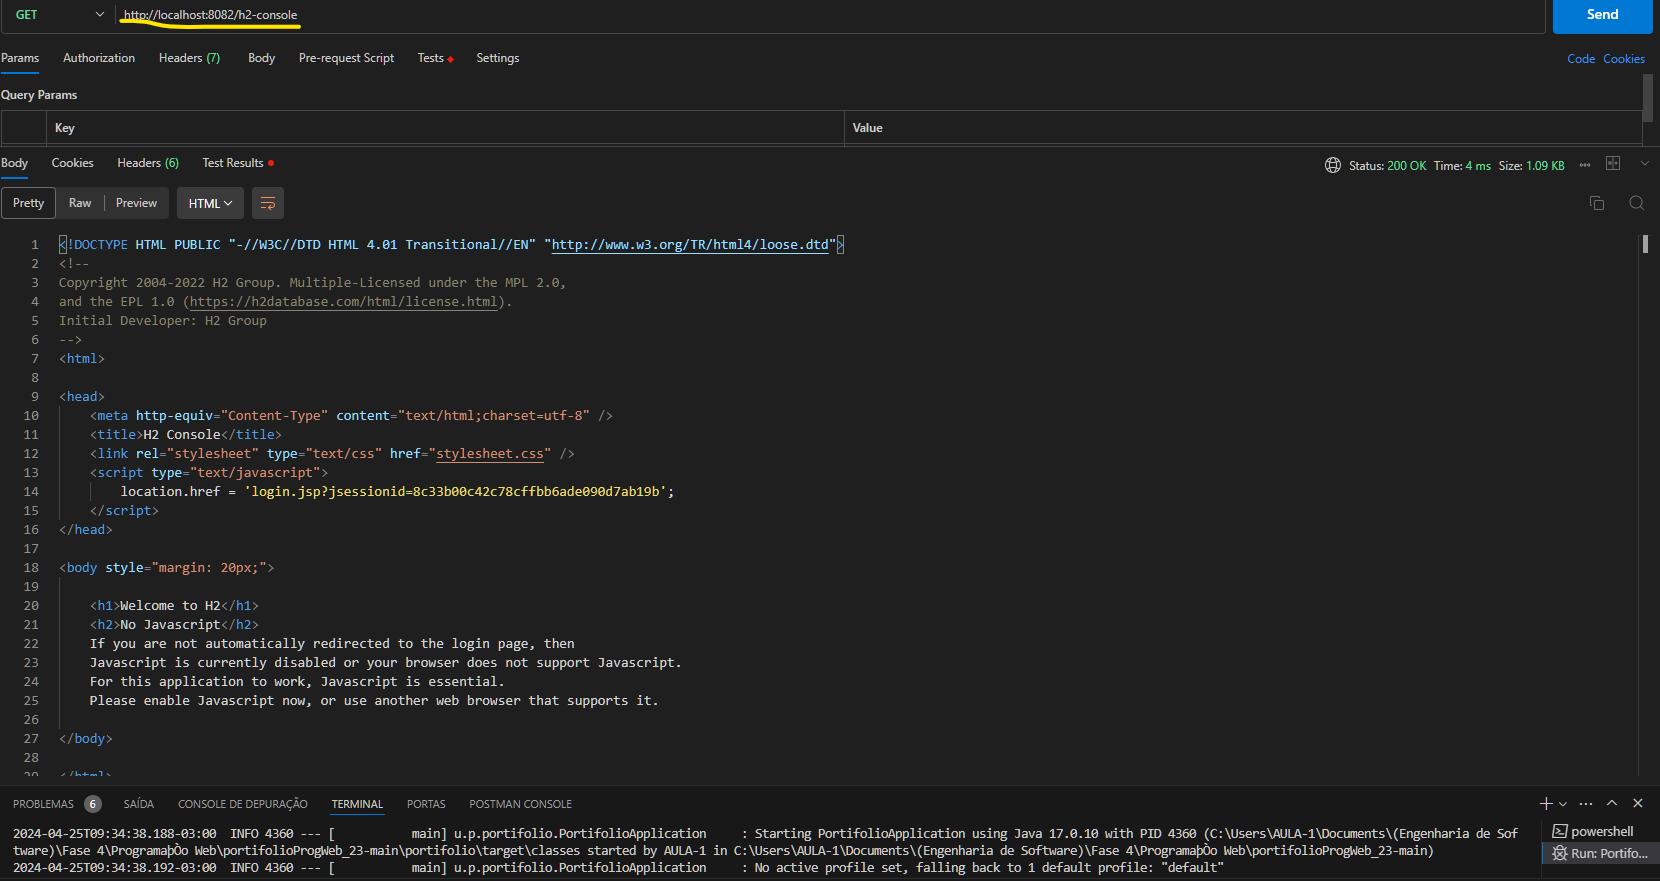
\includegraphics[width=\textwidth]{figure/postman_GET.png}
  \label{fig:get}
  \flushleft %esquerda
    {\fontsize{10pt}{\baselineskip}\selectfont
    Fonte: O autor (\the\year) }
\end{figure}

\begin{figure}[H]
\center
  \caption{Resultado do teste do postman com o POST.}
  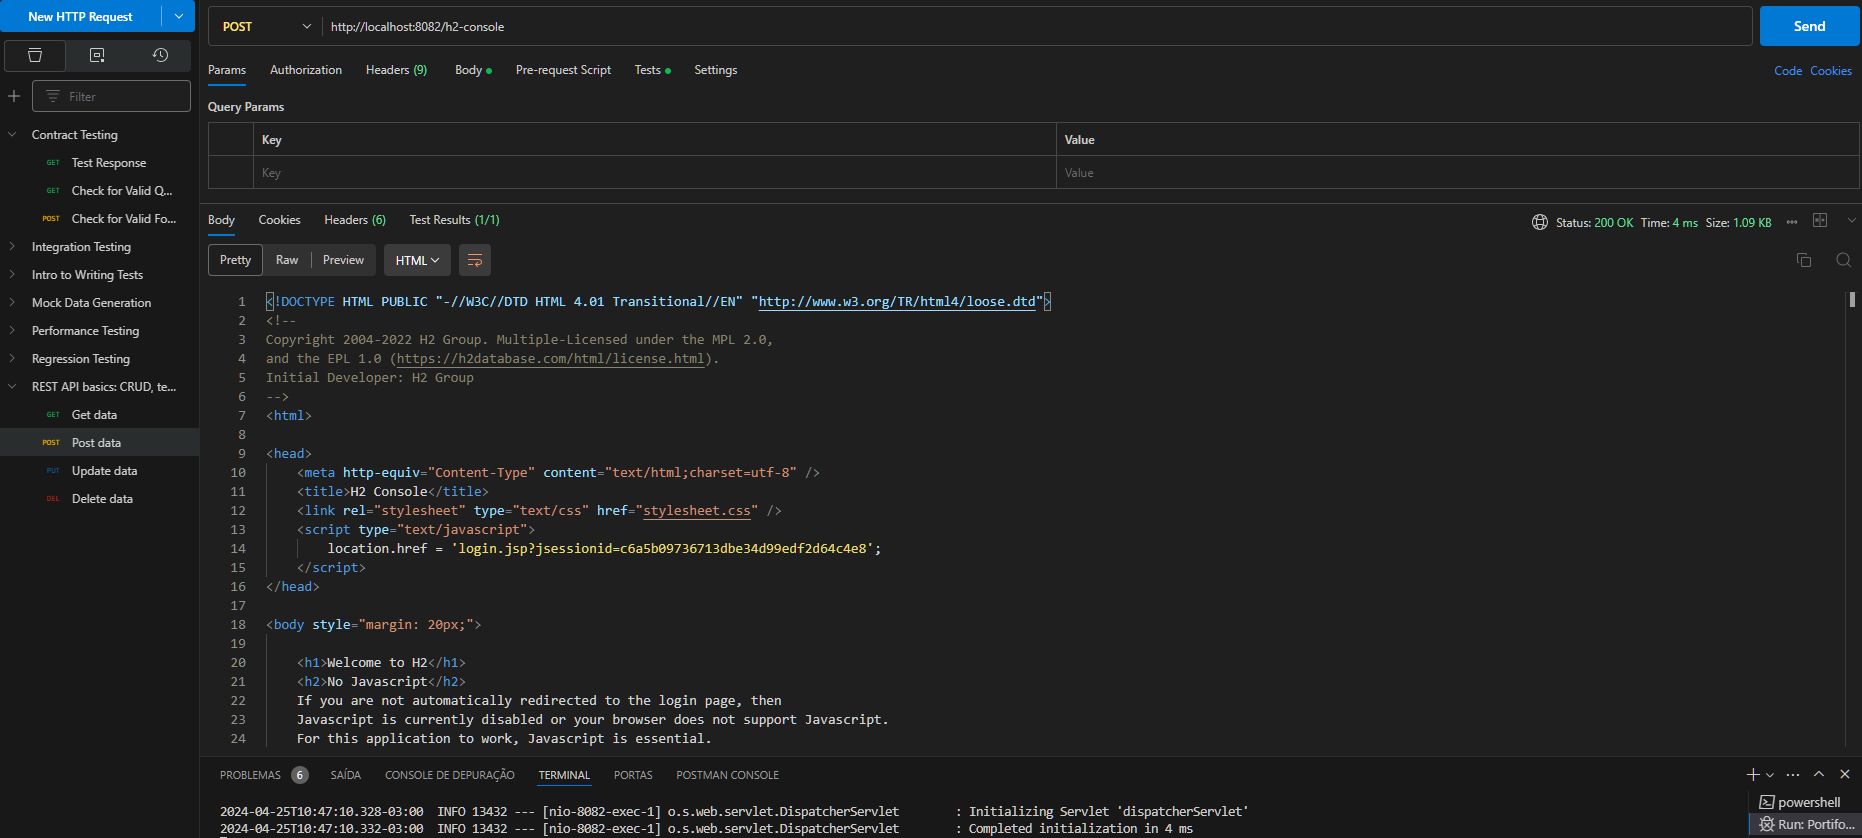
\includegraphics[width=\textwidth]{figure/postman_POST.png}
  \label{fig:post}
  \flushleft %esquerda
    {\fontsize{10pt}{\baselineskip}\selectfont
    Fonte: O autor (\the\year) }
\end{figure}


\par Podemos afereir a pagina exibina no navegador na figura \ref{fig:nav}.

\begin{figure}[H]
\center
  \caption{Resultado da tela de login.}
  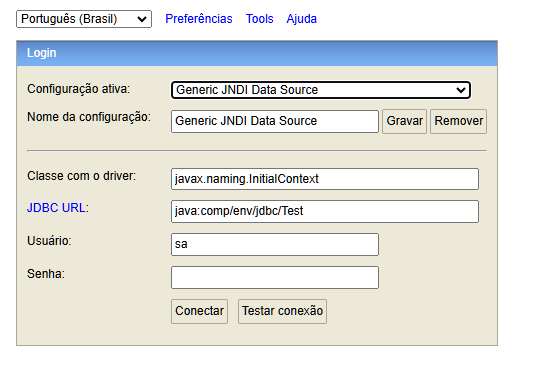
\includegraphics[width=\textwidth]{figure/login_nav.png}
  \label{fig:nav}
  \flushleft %esquerda
    {\fontsize{10pt}{\baselineskip}\selectfont
    Fonte: O autor (\the\year) }
\end{figure}


\subsection{Erro: novo usuário}

\par No roteiro da aula prática sugere a implementação do método \textbf{run}, da forma como esta exposto na listagem \ref{cod:userErro}. Na linha 19 e 20 na criação de um novo usuário é indicado o primeiro campo como \textit{\textbf{null}}, porém o mesmo não é aceito, conforme documentação.

\begin{figure}[H]
  \lstinputlisting[language=java, caption={Erro: novo usuário}, label={cod:userErro}]{errorUser.java} %Busca os codigos na pasta /cod
  \flushleft %esquerda
    {\fontsize{10pt}{\baselineskip}\selectfont  Fonte: O autor (\the\year) }
\end{figure}

\par Na figura \ref{fig:sugconstrutor}, a IDE expõe o que é esperado pelo construtor.

\begin{figure}[H]
  \caption{Argumentos demonstra que o construtor \textit{User} espera.}
  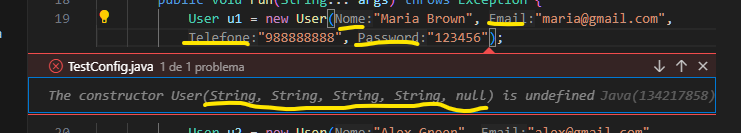
\includegraphics[scale=0.8]{figure/user_jaova.png}
  \label{fig:sugconstrutor}
  \flushleft %esquerda
  {\fontsize{10pt}{\baselineskip}\selectfont  Fonte: O autor (\the\year) }
\end{figure}
\par Desta forma, o código foi alterado para o que esta na listagem \ref{cod:user}.


\begin{figure}[H]
  \lstinputlisting[language=Java, firstline=18, lastline=20, caption={Construtor \textit{User}, alterado}, label={cod:user}]{TestConfig.java} %Busca os codigos na pasta /cod
  \flushleft %esquerda
  {\fontsize{10pt}{\baselineskip}\selectfont  Fonte: O autor (\the\year) }
\end{figure}



\section{Conclusões}
\par A realização desta aula prática é fundamental para pôr em prática os conteúdos adqueridos em sala de aula virtual, com estas ferramentas e viabilizado uma vivência do estudante mais próximo a realidade encontrada no mercado de trabalho, nesta aula em questão pude aferir que as tecnologias estão sempre em aprimoração, o caso prático é de que no roteiro sugeria a utilização de uma determinada versão do \textit{spring initialir}, porém a mesma não estava mais disponível, o mesmo caso acontece na listagem \ref{cod:userErro}, as bibliotecas vão sendo dia a dia aprimoradas e alguns aspectos são descontinuados ou alterados e esta vivência faz parte do profisional de desenvolvimento.
\par De igual modo com a eleboração desta aula prática pude explanara as divergências que encontrarei na vida profissional e que nem sempre serão flores, entretanto a dificuldade tem seu papel importante na construção do profissional, pois o obriga a deixar a zona de conforto.

  %$X \xLongleftarrow[\text{NATAN}]{\text{OGLIARI}} Y $ %COM TEXTO
	% $\uparrow$ %Seta para Cima
	%$\overleftarrow{NATAN}$
